% Design should cover the abstract design in such a way that someone else might be able to do what you did, 
% but with a different language or library or tool. This might include overall system architecture diagrams,
% user interface designs (wireframes/personas/etc.), protocol specifications, algorithms, data set design choices,
% among others. Specific languages, technical choices, libraries and such like should not usually appear in the design. These are implementation details.

\chapter{Design}

\section{Overview}
The design of the system can be broken down into a few fundamental categories:
\begin{itemize}
    \item 
        The foundational structure of the web app
        \begin{enumerate}
            \item Site structure
            \item Layout of the database
        \end{enumerate}
    \item 
        The three audio tracks which make up the system
        \begin{enumerate}
            \item The ambience mixer
            \item The 16-step sequencer
            \item The various instruments
        \end{enumerate}
    \item 
        The design of the interface
        \begin{enumerate}
            \item Visual design
            \item Sound design
        \end{enumerate}
\end{itemize}
This chapter will cover the key design choices in each of these categories and why they were chosen to fulfil the project’s requirements.

\section{App Foundations}

\subsection{Site Structure}
The site has two main pages plus additional accessory pages for the accounts system and the About page. Most of the site’s functions are on the “Room” pages, where users will interact with the audio systems. The homepage has links to all available rooms, and there are pages on the navigation bar (which is visible sitewide) for signing in, logging out, and registering a new account.

\subsection{Database Layout}
The database for this project is minimal and consists of a Room, Message, and User table.
\begin{itemize}
    \item 
        The Room table has a name and a many-to-many field containing the IDs of the users currently connected to it
    \item 
        The User table contains the username and password of the user alongside other generic information
    \item 
        The Message table contains messages the user has sent into a room and contains the user and room IDs, the content of the message, and the time it was sent
\end{itemize}
Each of the tables uses an auto-incrementing ID field as its primary key. Figure \ref{fig:erd} shows the entity-relationship diagram of the database.

\begin{figure}[htb]
    \centering
    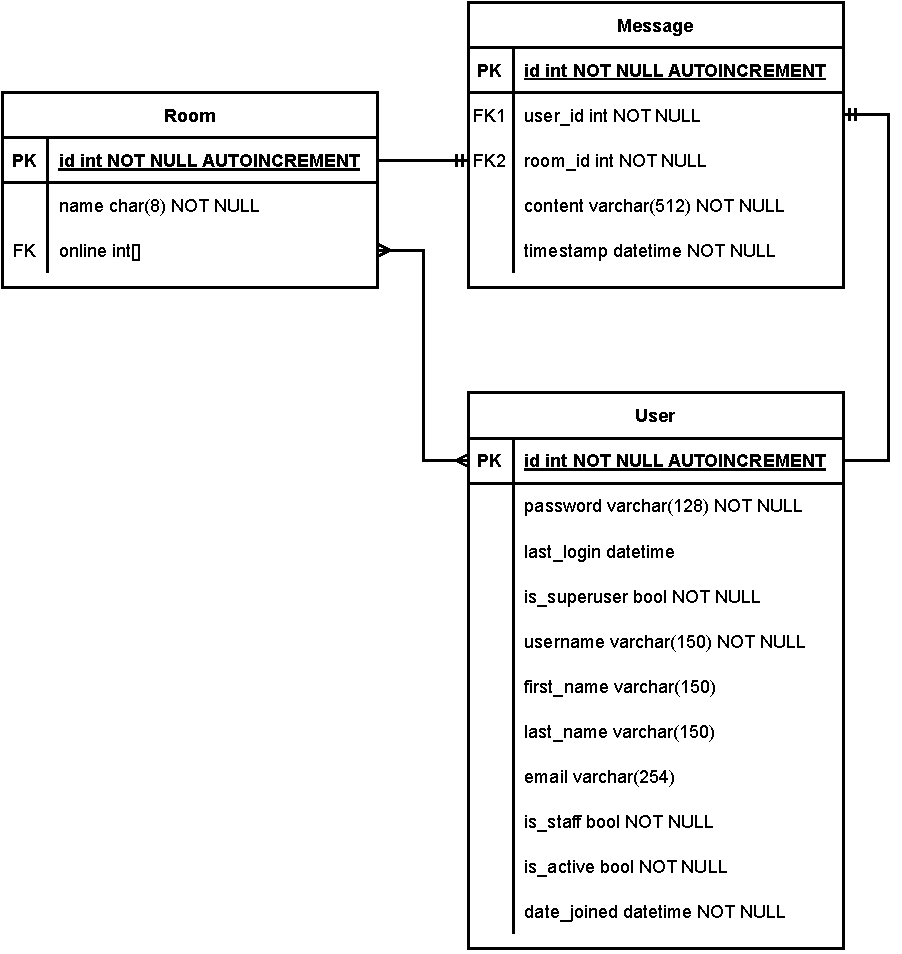
\includegraphics[width=0.5\linewidth]{images/design/entity-relation.pdf}    
    \caption{Entity-relationship diagram of the app's database}
    \label{fig:erd}
\end{figure}

Users register with a username and password. As this site’s user implementation is basic and only used to associate names with chat messages, no other information is required.


\section{Controlling the System}

The room page consists of three main panels, with each corresponding to an audio track. These tracks are:
\begin{itemize}
    \item The ambience mixer
    \item The 16-step sequencer
    \item The various instruments
\end{itemize}

This section will cover the design of each panel, and how certain design decisions were made to meet the requirements specification.

\subsection{Ambience Track}
The ambience panel will consist of a series of sliders which link to the volume of a certain ambient sound. This panel is designed to mimic real-world mixing desks which often include a series of vertical sliders to adjust the gain (volume) of a track. There will also be a mute toggle switch to quickly disable or enable that specific sound. Users will use these sliders to create an ambience mix or soundscape by combining multiple sounds in varying levels. Figure \ref{fig:mixer-design} compares the app's ambience panel to a real-world mixing desk.

\begin{figure}[htb] 
    \centering
    \begin{subfigure}[b]{0.45\textwidth}
        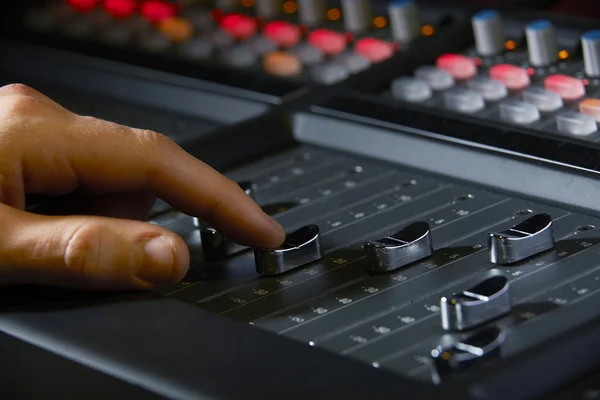
\includegraphics[width=\textwidth]{images/design/mixing-desk.png}
        \caption{The track sliders of a mixing desk, commonly found in recording studios. (Source: Depositphotos)}
        \label{fig:mixing-desk}
    \end{subfigure}
    ~
    \begin{subfigure}[b]{0.45\textwidth}
        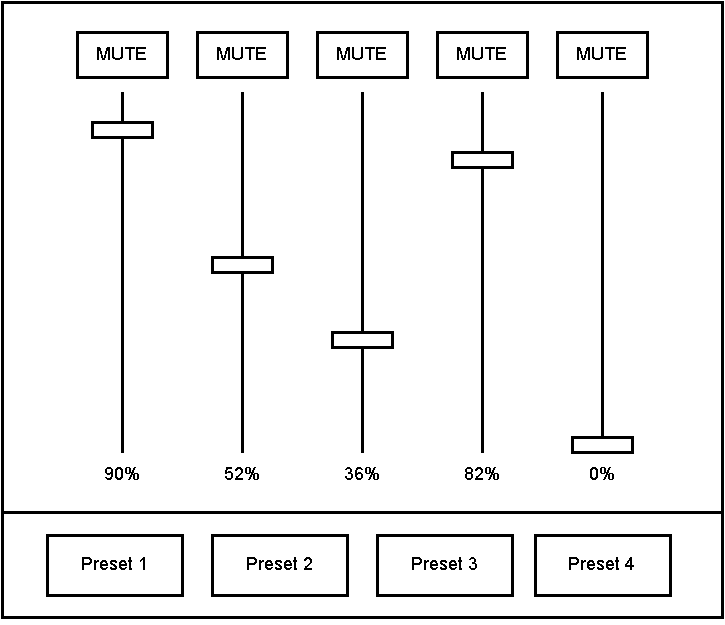
\includegraphics[width=\textwidth]{images/design/mixer-wireframe.pdf}
        \caption{Wireframe of the project's ambience page.}
        \label{fig:mixer-wireframe}
    \end{subfigure}
    ~
    \caption{
    The design of the \subref{fig:mixer-wireframe} ambience page takes after the real-world design of a \subref{fig:mixing-desk} mixing desk.
    }\label{fig:mixer-design}
\end{figure}

The sounds used for each track are similar to sounds available in existing ambient generator sites, for example, heavy thunder, a crackling fire, a recording of a coffee shop, and crickets chirping. These sounds were chosen because

In addition, there will be preset soundscapes which users can click on to slide the mixer to a pre-defined state. This is also similar to real-world mixing desks, where user-defined states can be saved and loaded, triggering the physical sliders to smoothly slide to that state. The mixer should emulate that sliding animation so that the transition between presets looks more realistic and natural, which benefits the user experience.

\subsection{Sequencer Track}
The sequencer panel primarily consists of a grid of buttons which represent the 16 timesteps across 8 different drum samples. When the buttons are clicked, they will light up to indicate that they are enabled. As the sequencer loops one column at a time through the timesteps from left to right (or steps 0 to 15), they will play any enabled sample at that given timestep. For example, in Figure \ref{fig:sequencer-wireframe}, in step 3, the sequencer will play the “Closed Hi-Hat” and “Crunch” samples, while in step 12, the “Kick” and “Snare” samples will play. Once the sequence reaches step 15, it resets back to step 0 and traverses the steps again. This is similar to existing implementations of online drum machines as well as real-world step sequencers.

\begin{figure}[htb]
    \centering
    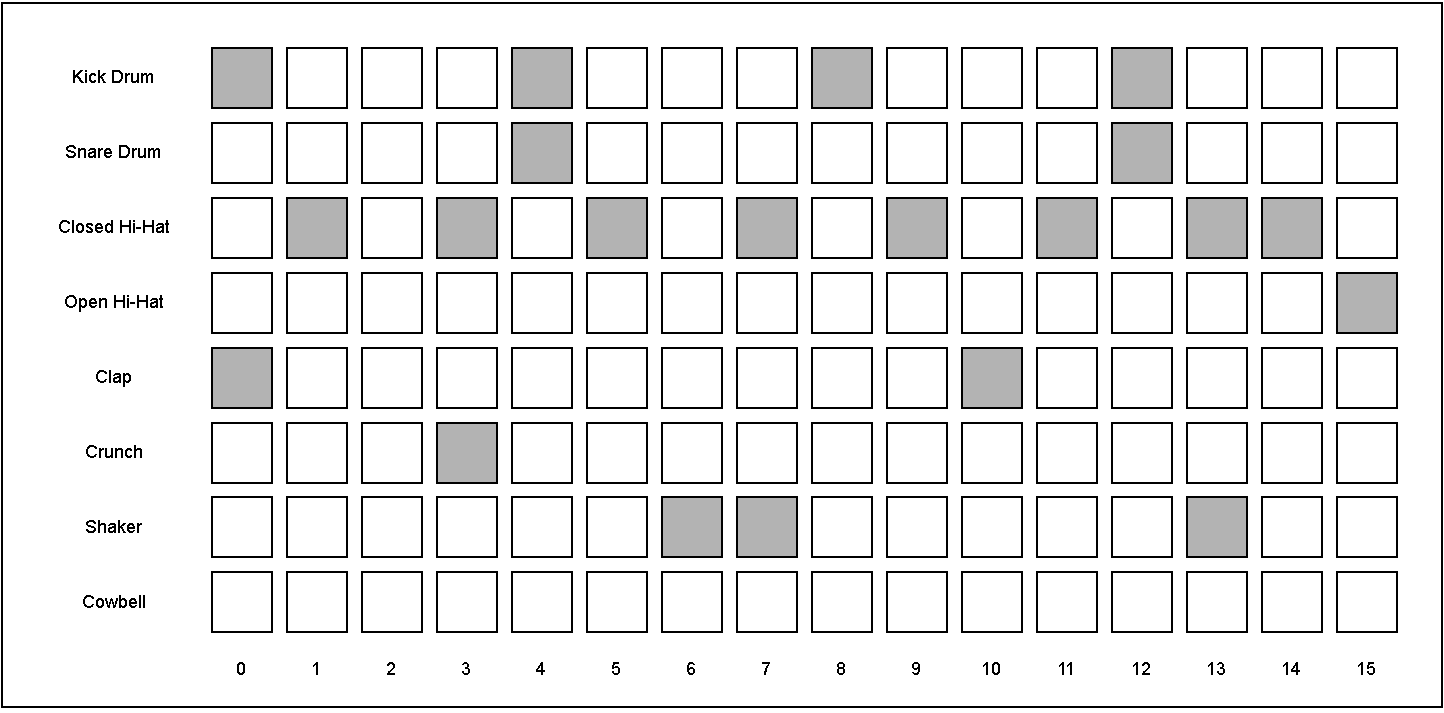
\includegraphics[width=0.8\linewidth]{images/design/sequencer-wireframe.pdf}    
    \caption{Wireframe of the project's sequencer page.}
    \label{fig:sequencer-wireframe}
\end{figure}

The chosen samples are popular percussion sounds and are commonly found in similar systems, such as kick and snare drums, cymbals, and claps. Additionally, the individual tracks will be able to be muted/unmuted to quickly turn on and off specific samples. There should also be a button to clear the sequencer, which turns off all active buttons.


\subsection{Instrument Track}
The instrument panel contains the different instruments that can be added to the mix, and their modifiers and parameters. Initially, this page was designed to use circular knobs to adjust the parameters as this more closely mimicked real-world controls, for example, the volume and tone knobs on an electric guitar (see Figure \ref{fig:guitar-knobs}). However, when testing these with a mouse it was more difficult to precisely control the levels of the parameters compared to the sliders used in the previous two panels. It also required a lot more custom scripting and event listeners compared to sliders, which are a built-in HTML element.

\begin{figure}[htb]
    \centering
    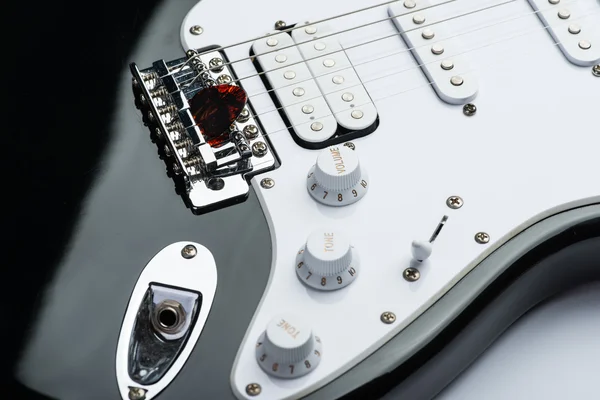
\includegraphics[width=0.5\linewidth]{images/design/guitar-knobs.png}    
    \caption{Electric guitars typically use twistable knobs to control their volume and tone (Source: Depositphotos).}
    \label{fig:guitar-knobs}
\end{figure}

Instead, sliders are used to adjust the parameters and modifiers of their corresponding instrument. Although this was not as aesthetically pleasing as using control knobs, it was more user-friendly and accessible for smaller devices due to the larger control surface enabling more precise adjustments. See the comparison between the two designs in Figure \ref{fig:instrument-wireframe}.

\begin{figure}[htb] 
    \centering
    \begin{subfigure}[b]{0.45\textwidth}
        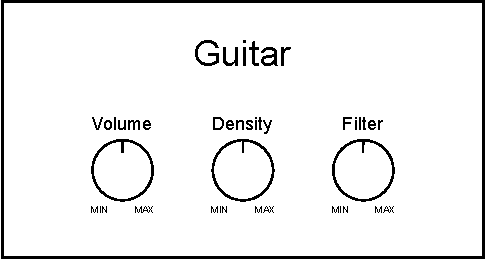
\includegraphics[width=\textwidth]{images/design/instrument-knob-wireframe.pdf}
        \caption{Wireframe of an instrument box using knobs.}
        \label{fig:instrument-knob-wireframe}
    \end{subfigure}
    ~
    \begin{subfigure}[b]{0.45\textwidth}
        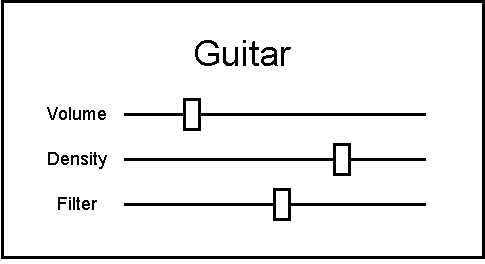
\includegraphics[width=\textwidth]{images/design/instrument-slider-wireframe.pdf}
        \caption{Wireframe of an instrument box using sliders.}
        \label{fig:instrument-slider-wireframe}
    \end{subfigure}
    ~
    \caption{
    Compared to \subref{fig:instrument-knob-wireframe} knobs, \subref{fig:instrument-slider-wireframe} sliders offer a larger control surface area.
    }\label{fig:instrument-wireframe}
\end{figure}

Each instrument will uniquely generate its part in real time, allowing users to adjust their parameters as the instrument plays. The instruments will be balanced so that they support each other compositionally, for example, some instruments will have the role of supporting the mix rhythmically by playing more steadily in an accompaniment style, while other instruments will have more of a lead role, generating melodies on top of the existing instrumentation.

According to the requirements specification, users should have sufficient control over the instruments so they feel like they are contributing significantly to the overall sound of a given session. There are two types of modifiers which will be used in this system: Filters, which modify the timbre or tone of the output sound, and generator parameters, which will change how the instruments pick which notes to play and when they play them. As the instruments play, the user can adjust their volume and any instrument-specific parameters. The implementation section will cover which instruments were added, and the behaviour of each.

All the instruments follow a similar behaviour, with the one exception of the guitar. Instead of picking a note or notes to play at a given timestep, the guitar is pre-programmed with a concrete set of MIDI recordings lasting two measures/bars of music each, where each phrase has an associated “intensity” and “density” label. For example, if the user sets the intensity to “medium” and the density to “sparse”, the guitar will randomly pick a pre-recorded phrase which is labelled with medium intensity and sparse density, playing that sample at the start of the next two measures.

The guitar is defined this way to allow for greater expressive control over the instrument, allowing pitch bends, vibrato, and more complex rhythmic phrasing to be included in the samples, which would not be possible if the guitar used the same system as the other instruments.

\subsection{Integrating Tracks}
The three audio tracks are designed to integrate seamlessly and harmoniously to create a cohesive and continuous musical composition. The ambience track plays continuously, with the sounds perpetually looping to create an auditory backdrop to the sound mix. The sequencer and instrument tracks are triggered simultaneously and follow a pulse which is sent from the server to each client, allowing the drums to play perfectly in time with the instruments.


\section{Interface Design}

\subsection{Navigation between Panels}
To navigate between the three track panels, there will be a navigation bar. When the page loads, the panels will be hidden apart from the ambience panel which is open by default. Then, when the user clicks on a panel the current panel will fade out while the new panel fades in. The room page will use this layout to simplify the appearance of the app and not overwhelm the user with options and controls. Additionally, one panel is visible at a time on purpose so that when multiple users are using the system, one user can be controlling one panel while another user can be controlling a separate panel. This should encourage collaboration since a user can only control one track at a given time.

The navigation bar (Figure \ref{fig:navigation-wireframe}) also doubles as a master mixer, as there will be volume sliders which control the master volume for its associated track.

\begin{figure}[htb]
    \centering
    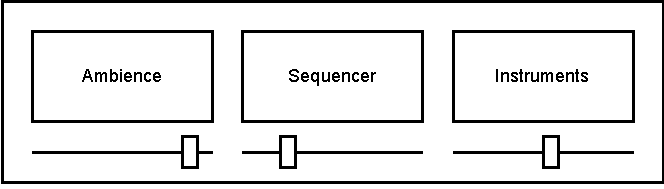
\includegraphics[width=0.5\linewidth]{images/design/navigation-wireframe.pdf}    
    \caption{Wireframe for the navigation bar with master volume sliders underneath each track.}
    \label{fig:navigation-wireframe}
\end{figure}

\subsection{Visual Design}
As mentioned previously, much of the design purposely mimics existing real-world technologies and systems, such as mixing desk sliders and step sequencer button grids. Known as “Skeuomorphism”, this design style has been proven in a study by \cite{urbano2022skeuomorphism} to be more effective and accurate at conveying interface elements which can be clicked or interacted with when compared to more flat or minimalist designs. Skeuomorphism is commonplace amongst music production software, an example of which can be seen with audio compressor plugins in Figure \ref{fig:compressor}.

In addition to using skeuomorphic-inspired design, adding visual cues like changing the colour or size of interface elements when users hover their mouse cursor over them also helps to indicate when an element can be interacted with, so these cues will be in place for all of the interactable controls in the system.

\begin{figure}[htb] 
    \centering
    \begin{subfigure}[b]{0.45\textwidth}
        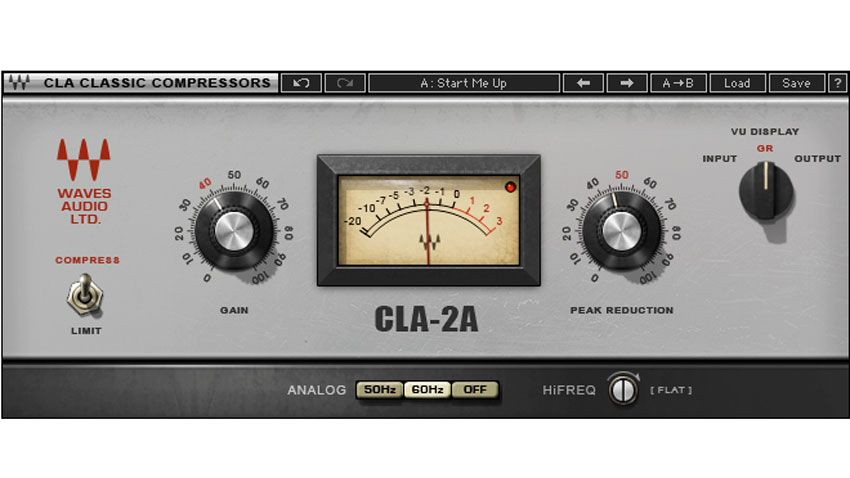
\includegraphics[width=\textwidth]{images/design/compressor-digital.png}
        \caption{A digital compressor plugin for a DAW. (Source: Waves Audio)}
        \label{fig:compressor-digital}
    \end{subfigure}
    ~
    \begin{subfigure}[b]{0.45\textwidth}
        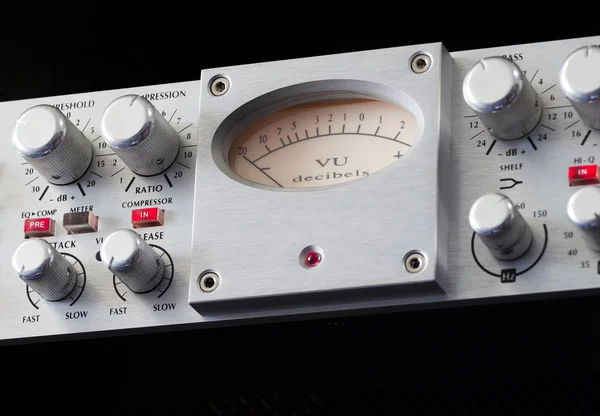
\includegraphics[width=\textwidth]{images/design/compressor-analogue.png}
        \caption{A physical analogue compressor. (Source: Depositphotos)}
        \label{fig:compressor-analogue}
    \end{subfigure}
    ~
    \caption{
    Digital music production plugins like \subref{fig:compressor-digital} often mimic the look and feel of physical analogue units like \subref{fig:compressor-analogue}. 
    }\label{fig:compressor}
\end{figure}

\subsection{Sound Design}
In addition to the system’s visual design. The user experience can be positively affected by the sound design of the app. Providing immediate auditory feedback confirms that their action has been recognised by the system and helps build their confidence in interacting with the interface. It has also been proven to help reduce cognitive load as users can rely on auditory cues to confirm their actions. One particular study by \cite{jeon2015menu} found that adding auditory cues to a car’s infotainment system resulted in a lower perceived workload when executing tasks such as scrolling through music playlists. This allowed drivers to operate menus more efficiently while driving more safely. This is important to create a relaxing atmosphere and immerse the user as they can pay more attention to the music-making experience.

Some examples of these cues are button-pressing sounds when the user clicks on a toggle switch, or notch sounds when the user interacts with a slider control. Similarly to the visual design, these sounds will be chosen to mimic real-world interactions with controls such as buttons, switches, and mixer sliders. A study by \cite{sikora1995musical} found that real-world sounds mapped more reliably and predictably to corresponding GUI functions compared to more abstract auditory cues. Therefore, by incorporating real-world sounds into the interface, the system’s design can leverage users’ existing mental models, making it easier for them to interpret the auditory feedback.
